\documentclass{article}
\usepackage[a4paper, top=4cm, bottom=4cm, left=35mm, right=35mm]{geometry} % Modification des tailles des marges (on en parlera après).

% Gestion des polices en fonction de l'encodage (PDFLaTeX, XeLaTeX, LuaTeX ou autre) :
\usepackage{ifxetex}
\usepackage{mathtools}
\usepackage{amssymb}
\usepackage{ifluatex}
\ifxetex
  % XeTeX est utilisé :
  \usepackage{fontspec}
\else
  \ifluatex
    % LuaTeX est utilisé :
    \usepackage{fontspec}
  \else
    % pdfLaTeX ou autre moteur est utilisé :
    \usepackage[T1]{fontenc}
    \usepackage[utf8]{inputenc}
    \usepackage{lmodern}
  \fi
\fi

% Autres packages :
\usepackage[french]{babel}
\usepackage{mdframed}
\usepackage{enumitem}
\usepackage{hyperref}
\usepackage{amsmath}
\usepackage{amsfonts}
\usepackage{stmaryrd}
\usepackage[explicit]{titlesec}
\usepackage{framed}
\usepackage{amsthm}
\usepackage{bbm}
\usepackage{xcolor}
\usepackage{tcolorbox}
\tcbuselibrary{breakable}
% Package permettant de générer des graphes :
\usepackage{tikz}
\usetikzlibrary{arrows}
\usetikzlibrary{arrows.meta}
\usepackage{pgfplots}
\pgfplotsset{compat=1.18} % Préciser la version de pgfplots afin qu'il soit compatible avec le type de document (ici "article").
%package pour images
\usepackage{graphicx}
\graphicspath{ {./ressources/} }

\usepackage{pythonhighlight}

\sloppy % Pour que les URLs ne dépassent pas des marges.

\title{Algorithme d'Hastings-Metropolis - Problème du voyageur de commerce}
\author{PEROTTINO Tony, LE BER Tom, \\ VAILLANT Corentin et BERNARD Léo}

\begin{document}
\maketitle

\newpage
\tableofcontents
\newpage

\section*{Préambule}

Ce rapport s'inscrit dans le cadre de la matière "Projet de Mathématiques" de l'université de Toulouse (Paul Sabatier). \\
L'objectif de ce rapport est de présenter et de prouver l'algorithme d'Hastings-Metropolis. À la fois d'expliquer en détail son fonctionnement, mais aussi de comprendre l'intérêt qu'il présente dans les sciences et en quoi il prend sa valeur. \\
Pour illustrer l'algorithme, nous nous intéresserons au problème du voyageur de commerce et étudierons sa complexité.


\section{Introduction}

Afin de comprendre en profondeur ce sujet, il est nécessaire de s'en faire une idée globale, même naïve, pour pouvoir suivre convenablement la ligne directrice de notre discours.

\subsection{Informations générales et description historique}

L'algorithme d'Hastings-Metropolis (noté "HM" dans ce rapport) consiste en une méthode d'échantillonnage stochastique permettant, à partir d'une distribution de probabilité donnée, de pouvoir décrire son comportement et d'obtenir des statistiques dessus. Cet algorithme prend sa valeur quand la distribution est difficile à analyser (systèmes multidimensionnels, par exemple) et permet de résoudre de nouveaux problèmes avec une complexité temporelle décente. \\
Cette méthode est marquante, car elle a été conceptualisée tôt dans l'histoire de l'informatique et a mis des décennies avant d'être prouvée et expliquée entièrement. \\

Historiquement, c'est en 1949 que l'écriture de l'algorithme a été publiée dans un article de Nicholas Metropolis et Stanisław Ulam. La paternité de l'algorithme est soumise à débat, car l'algorithme s'inscrit sous le nom de son chef de projet (Metropolis), alors que l'équipe composée de Nicholas Metropolis, Arianna et Marshall Rosenbluth, Augusta et Edward Teller a contribué à cette méthode. Ils étudiaient alors plus particulièrement le cas de la distribution de Boltzmann, une des distributions les plus utilisées en physique statistique, dans des travaux datant de 1953. \\
Cela illustre une dynamique fréquente dans les sciences, où le mérite est disproportionnellement attribué à une personne alors qu'il s'agit des efforts de toute une équipe. En particulier, Arianna Rosenbluth était considérée comme brillante par le monde scientifique. \\

En 1970, W. K. Hastings (1930-2016) a étendu l'algorithme au cas d'une distribution quelconque, et c'est cette version généralisée qui est connue sous le nom d'algorithme d'Hastings-Metropolis. Cette extension a eu de nombreuses applications dans divers domaines scientifiques, comme en statistique bayésienne (espaces complexes multidimensionnels), en biologie computationnelle (analyse des séquences génétiques), en économie et en finance (modèles stochastiques MCMC en général), etc. \\

Quant à lui, le problème du voyageur de commerce (dit "TSP", comme Travelling Salesman Problem en anglais) est un problème classique et bien connu pour être un problème NP-difficile, ce qui signifie qu'il n'existe actuellement aucune méthode connue capable de le résoudre de manière optimale en temps polynomial pour toutes les tailles d'instances, et qu'il est au moins aussi difficile que les problèmes de NP. 
L'origine du problème est assez incertaine : il a été formulé pour la première fois vers 1850 dans un manuel d'un commerçant voyageant en Suisse et en Allemagne. Ce n'est que dans les années 1930 que le problème fut énoncé d'abord comme un casse-tête (par William Rowan et Thomas Kirkman), puis étudié (par, entre autres, Thomas Kirkman, Jillian Beardwood, J. H. Halton et John Hammersley). \\ 
Le problème consiste à déterminer le chemin le plus court passant par tous les points d'un graphe une seule fois chacun, en terminant par le point de départ (recherche d'un cycle hamiltonien le plus court). Les distances peuvent être dites symétriques ou asymétriques, c'est-à-dire que la distance entre eux varie en fonction de la direction du déplacement. On peut illustrer ce problème grâce à un voyageur de commerce devant vendre ses produits dans chacune des villes en un minimum de temps. Ce problème peut donc être naturellement représenté par un graphe.\\

\subsection{Pourquoi HM permet-il de résoudre le problème du voyageur de commerce ?}

Le principe mathématique derrière HM repose sur la construction dynamique d'une chaîne de Markov, qui n'est pas connue au préalable mais se développe au fil des itérations. À mesure que l'algorithme progresse, le comportement de cette chaîne converge vers la distribution cible, permettant d'obtenir un échantillon fiable de solutions par rapport aux états de la distribution. \\
Quant au problème du voyageur de commerce, il peut être représenté par un graphe orienté ayant un sommet pour chaque ville et une arête pour chaque temps de trajet. Nous verrons par la suite qu'une chaîne de Markov peut être associée à un graphe orienté, c'est-à-dire que le problème du voyageur de commerce est résoluble par HM. \\
Par résoluble, il est important de préciser qu'il s'agit d'une résolution approximative parce que le TSP est NP-difficile comme mentionné précédemment.
En conséquence, l'objectif de HM n'est pas d'apporter la réponse exacte au problème, mais une approximation fiable de la solution, ce qui peut sembler contre-intuitif. Cette approximation est la caractéristique principale des méthodes MCMC que nous aborderons dans leur partie dédiée. \\

Il convient de souligner que, dans le cas du TSP, c'est à la version d'optimisation que l'on s'intéresse, par opposition au problème décisionnel, qui, lui, est NP-complet. La différence entre ces deux formulations repose sur leur objectif : dans le TSP décisionnel, on pose une question du type "Existe-t-il un chemin de coût inférieur ou égal à une valeur donnée ?", à laquelle il s'agit de répondre par oui ou non.
Alors que le TSP d'optimisation cherche à partir de la situation initiale la meilleure solution : donc optimiser le chemin au fil des itérations. C'est cette version du problème pour laquelle l'approche par échantillonnage stochastique est envisageable.
Précisons toutefois que HM n'est habituellement pas la méthode que l'on utilise pour le TSP en pratique. Usuellement, le nombre de ville étant grand (suffisamment pour que la solution par brute force ne soit pas trouvable) mais pas absurde (une centaine par exemple), on préfère utiliser des versions déterministes optimisées comme l'algorithme de Held-Karp de complexité $O(2^n \times n^2)$, ou dans le cas de situation avec encore plus de villes, des méthodes similaires à HM plus adaptées comme l'échantillonnage de Gibbs.

En somme, il est important de comprendre que HM est un outil adapté à la résolution de problèmes dont l'espace des solutions est trop vaste pour être exploré exhaustivement dans un temps raisonnable. C'est donc par l'approximation de la solution optimale, à travers des échantillons, que cette méthode permet de trouver une solution satisfaisante.
Cette nuance est essentielle, car elle met en lumière la sophistication de HM en tant qu'outil d'approximation pour des problèmes complexes.

\subsection{Objectif de ce rapport}

L'objectif de ce rapport étant d'apporter une solution fiable au TSP grâce à HM, nous prouverons alors le fonctionnement dde ce dernier grâce à la théorie mathématique des chaînes de Markov. Nous en expliciterons les définitions et propriétés fondamentales dans un premier temps, qui permettront de prouver l'algorithme d'HM dans un second temps. Nous présenterons alors à la fin du rapport une implémentation personnelle de l'algorithme.

\section{Chaînes de Markov à états finis}

\subsection{Définitions fondamentales}

\begin{tcolorbox}[colback=white,colframe=blue!80!black,title=Temps Discret et Temps Continu]
Soit $T$ un ensemble d'indices numérotées représentant le temps. \\

Il existe deux types de modélisation temporelle :
\begin{enumerate}[leftmargin=5em, label=(\arabic*)]
    \item Un processus \textbf{à temps discret} signifie que l'on considère les valeurs de la modélisation comme espacées régulièrement dans le temps.
          On peut prendre des ensembles dénombrables comme $T = \mathbb{N}$ ou $T = \mathbb{Z}$ où chaque instant est distinct.
    \item Un processus \textbf{à temps continu} signifie que $T$ n'est pas dénombrable. Il existe toujours un temps intermédiaire entre deux indices de $T$.
          Cela signifie que le processus évolue en tout instant dans un continuum temporel, on peut prendre des ensembles non dénombrables comme $T = \mathbb{R}_+$ où chaque instant est continu.
\end{enumerate}
\end{tcolorbox}

Dans ce rapport nous nous intéresserons uniquement au temps discret, pour pouvoir modéliser le problème du voyageur de commerce.
De plus, cette distinction joue un rôle fondamental dans la classification et l'analyse des \textbf{processus stochastiques} et n'implique pas les mêmes théorèmes. \\

\begin{tcolorbox}[colback=white,colframe=blue!80!black,title=Processus Stochastique]
Soit $(\Omega, \mathcal{F}, \mathbb{P})$ un espace de probabilité.

Soit $T$ un ensemble d'indices discret ou continu (souvent $T = \mathbb{N}$ ou $\mathbb{R}_+$). \\

Un \textbf{processus stochastique} est une famille de variables aléatoires $\{X_t\}_{t \in T}$ définies sur $(\Omega, \mathcal{F}, \mathbb{P})$ et à valeurs dans un espace d'états $E$ (appelé espace d'états du processus).
\end{tcolorbox}

Un processus stochastique permet de modéliser un système évoluant de manière aléatoire en fonction du temps.

Différents types de processus peuvent être étudiés en fonction des propriétés de dépendance temporelle et de la nature de l'espace d'états $E$.
Au cours de ce rapport, nous nous concentrerons l'un des principaux processus stochastiques à temps discret et à espace d'états fini ; les \textbf{chaînes de Markov}. \\

\begin{tcolorbox}[colback=white,colframe=red!80!black,title=Chaîne de Markov]
Soit $E$ un ensemble fini ou dénombrable.

Soit $(X_n)_{n \in \mathbb{N}}$ une suite de variables aléatoires à valeurs dans l'espace d'états $E$. \\

$(X_n)_{n \in \mathbb{N}}$ est appelée \textbf{chaîne de Markov} si et seulement si :
\begin{enumerate}[leftmargin=5em, label=(\arabic*)]
    \item Sa loi de probabilité initiale $X_0$ est bien définie.
    \item Elle respecte la \textbf{propriété de Markov}, telle que :
\end{enumerate}
\[
\forall n \in \mathbb{N}, \quad \forall x_0, x_1, \dots, x_{n+1} \in E,
\]
\[
\mathbb{P}(X_{n+1} = x_{n+1} \mid X_0 = x_0, \dots, X_n = x_n) = \mathbb{P}(X_{n+1} = x_{n+1} \mid X_n = x_n).
\]
\end{tcolorbox}

Une chaîne de Markov est un processus de Markov à temps discret ou à temps continu et à espace d'états discret. Un processus de Markov est un processus stochastique possédant la propriété de Markov : l'information utile pour la prédiction du futur est entièrement contenue dans l'état présent du processus et n'est pas dépendante des ses états antérieurs.

Autrement dit, la loi de probabilité $\mathbb{P}$ régissant la transition de l'état présent $X_n$ vers l'état futur $X_{n+1}$ dépend uniquement du dernier terme $X_n$, et reste totalement indépendante des tous ses états antérieurs $\{X_0, X_1, \dots, X_{n-1}\}$.

Cette propriété, que l'on peut qualifier de « sans mémoire » ou de propriété de Markov, constitue la caractéristique fondamentale de ces processus stochastiques. \\

\begin{tcolorbox}[colback=white,colframe=blue!80!black,title=Chaine de Markov Homogène]
Une chaîne de Markov est dite homogène quand $\forall n \in \mathbb{N}$, $\forall i,j \in E$ :
\[
  \mathbb{P}[X_{n+1} = j \mid X_n = i] = \mathbb{P}[X_1 = j \mid X_0 = i].
\]
\end{tcolorbox}

En somme, une chaîne de Markov homogène ne dépend pas des états précédents (propriété de Markov) et garantit que son comportement reste inchangé au fil du temps, c'est-à-dire que les probabilités de transition restent constantes quelque doit $t \in T$ (homogénéité de la chaîne de Markov). \\
Dans ce rapport, toutes les chaînes de Markov seront considérées comme homogènes. \\

\newpage % TODO
\subsection{Propriétés fondamentales}

% TODO
% Propriétés à parler : 
% - [X] Matricer de transition
% - [X] Lien avec les graphes orientés
% - [X] Propriétés en n-pas

\subsubsection{Matrice de Transition}

\begin{tcolorbox}[colback=white,colframe=red!80!black,title=Matrice de Transition]
Soit $(X_n)_{n \in \mathbb{N}}$ une chaîne de Markov homogène à temps discret à valeurs dans un espace d'états $E$, fini ou dénombrable. \\

$(X_n)_{n \in \mathbb{N}}$ est entièrement caractérisée par sa \textbf{matrice de transition} $P = (P_{i,j})_{i,j \in E}$, où chaque terme représente la probabilité de passer de l'état $i$ à l'état $j$ en une étape :
\[
\forall n \in \mathbb{N}, \quad \forall i,j \in E, \quad P_{i,j} = \mathbb{P}(X_{n+1} = j \mid X_n = i).
\]

Lorsque l'ensemble des états $E$ est fini, par exemple $E = \{1, 2, \dots, N\}$, la matrice $P$ s'écrit sous la forme :
\[
    P = \begin{bmatrix}
        P_{11} & P_{12} & \cdots & P_{1N}\\[1mm]
        P_{21} & P_{22} & \cdots & P_{2N}\\[1mm]
        \vdots & \vdots & \ddots & \vdots\\[1mm]
        P_{N1} & P_{N2} & \cdots & P_{NN}
    \end{bmatrix}
\]
\end{tcolorbox}

\begin{tcolorbox}[colback=white,colframe=blue!80!black,title=Matrice stochastique par lignes/colonnes]
Une matrice \textbf{stochastique par lignes} (appelée aussi \textbf{stochastique à droite}) est une matrice dont la somme des probabilités de ses lignes vaut 1 chacune et toutes ses probabilités sont positives :
\[
\forall i, \quad \sum_{j=1}^{N} P_{i,j} = 1 \quad \text{et} \quad 0 \leq P_{i,j} \leq 1.
\]

Respectivement, une matrice est \textbf{stochastique par colonnes} (dite aussi \textbf{stochastique à gauche}) lorsque :
\[
\forall j, \quad \sum_{i=1}^{N} P_{i,j} = 1 \quad \text{et} \quad 0 \leq P_{i,j} \leq 1.
\]
Une matrice est dite \textbf{bistochastique} lorsqu'elle est à la fois stochastique par lignes et par colonnes.
\end{tcolorbox}

Dans le cadre des chaînes de Markov homogènes, toutes les matrices de transition $P$ sont stochastiques par lignes car les probabilités de transition depuis chaque état sont normalisées (chaque ligne représentant le vecteur des probabilités de transition depuis un état donné vers l'ensemble des autres états). C'est-à-dire que la somme des probabilités pour passer d'un état à un autre vaut 1. \\

De manière analogue, si l'espace des états est infini dénombrable (par exemple $E = \{1, 2, 3, \dots\}$), on indexe les états de la même façon et la condition suivante reste valable :
\[
\forall i \in E, \quad \sum_{j \in E} P_{i,j} = 1.
\]

\subsubsection{Représentation sous forme de Graphe Orienté}
\label{subsubsec: Représentation sous forme de graphe orienté}

\begin{tcolorbox}[colback=white,colframe=red!80!black,title=Graphe Orienté d'une Chaîne de Markov]
Une chaîne de Markov homogène peut toujours être représentée sous forme d'un graphe orienté $ G = (V, A) $, où :
\begin{enumerate}[leftmargin=5em, label=(\arabic*)]
    \item $V$ est l'ensemble des sommets, correspondant à l'ensemble des états de l'espace d'états $E$.
    \item $A$ est l'ensemble des arcs, où chaque arc possède une pondération correspondant à la probabilité de transition $P_{i,j}$. Un arc de $i$ vers $j$ est représenté que si $P_{i,j} > 0$.
\end{enumerate}
\end{tcolorbox}

Représenter graphiquement une chaîne de Markov homogène permet de clarifier visuellement les différentes dynamiques de transitions entre chaque état du système et de comprendre la structure du processus stochastique. \\

\begin{tcolorbox}[colback=white,colframe=yellow!80!black,title=Exemple, breakable]
Considérons par exemple une chaîne de Markov ayant trois états $i, j, k$, ordonnés respectivement, et dont la matrice de transition est donnée par :

\begin{center}
$
P = \begin{bmatrix}
0.1 & 0.4 & 0.5 \\
0.6 & 0.4 & 0 \\
0.1 & 0.1 & 0.8 \\
\end{bmatrix}
$
\end{center}

Dans cette configuration, la probabilité de transition de l'état $i$ vers l'état $j$ est donnée par :
\[
P_{i,j} = P_{1,2} = \mathbb{P}(X_{n+1} = j \mid X_n = i) = 0.4
\]

% TODO
\newpage % /!\ TEMPORAIRE /!\ - Pour une bonne mise en page de l'exemple.
Nous obtenons ainsi le graphe suivant :

\begin{center}
\begin{tikzpicture}[
    >={Latex[length=3mm, width=2mm]},
    node distance=2cm,
    state/.style={circle, draw, minimum size=0.5cm, font=\large},
    every edge/.append style={draw, -latex, font=\small}
]

% Nodes :
\node[state] (A) at (0, 0) {$i$};
\node[state] (B) at (2, 3) {$j$};
\node[state] (C) at (4, 0) {$k$};

% Edges :
\draw[->] (A) edge[loop left, out=150, in=210, looseness=8] node[left] {0.1} (A);
\draw[->] (A) edge[bend right=20] node[left] {0.4} (B);
\draw[->] (A) edge[bend right=16] node[below] {0.5} (C);

\draw[->] (B) edge[bend right=20] node[left] {0.6} (A);
\draw[->] (B) edge[loop above, out=60, in=120, looseness=8] node[above] {0.4} (B);

\draw[->] (C) edge[bend right=16] node[below] {0.1} (A);
\draw[->] (C) edge[bend right=20] node[right] {0.1} (B);
\draw[->] (C) edge[loop right, out=330, in=30, looseness=8] node[right] {0.8} (C);

\end{tikzpicture}
\end{center}
\end{tcolorbox}

\subsubsection{Matrice de transition en \texorpdfstring{$k$}{k}-pas} % Pour que "hyperref" supporte l'expression mathématique "$k$" dans la chaîne de caractère générant un des signets du PDF.
\label{subsubsec: Matrice de transition en k-pas}

\begin{tcolorbox}[colback=white,colframe=red!80!black,title=Matrice de transition pour $k$-transitions]
Soit $(X_n)_{n \in \mathbb{N}}$ une chaine de Markov homogène d'espace d'états $E$ fini ou dénombrable tel que $\left\{1,2,\ldots,N\right\}$. On note $P$ sa matrice de transition. \\

Pour tout état $E_i$ et $E_j$ et pour tout entier naturel $k \geq 1$, le coefficient de la ligne $i$ et de la colonne $j$ de \textbf{la matrice $P^k$ est la probabilité de passer de l'état $E_i$ à celui $E_j$ en $k$ transitions}.
\end{tcolorbox}

Les chaînes de Markov homogènes permettent de déterminer l'état d'un système après $k$ transitions, c'est-à-dire au bout du $k$-ième mouvement dans la chaine, en élevant la matrice de transition à la puissance $k$. \\
Plus formellement, on a :
\[
P_{i,j}^{(k)} = \mathbb{P}(X_k = j \mid X_0 = i).
\]
Ce résultat vient de la propriété de Markov, qui indique que la probabilité de transition d'un état $i$ à un état $j$ dépend uniquement du dernier pas réalisé, et non de tous les précédents.

\begin{tcolorbox}[colback=white,colframe=green!80!black,title=Démonstration]
La démonstration de cette propriété passe par celle de l'\textbf{équation de Chapman-Kolmogorov}, telle que $\forall i,j \in E$ et $\forall n,m \in \mathbb{N}$ :
\[
\mathbb{P}(X_{n+m} = j \mid X_0 = i) = \sum_{k \in E} \mathbb{P}(X_{m} = j \mid X_0 = k) \cdot \mathbb{P}(X_n = k \mid X_0 = i).
\]

Ce qui équivaut en termes matriciels :
\[
P_{i,j}^{(n+m)} = \sum_{k \in E} P_{i,k}^{(n)} \cdot P_{k,j}^{(m)}.
\]

Cette relation peut s'interpréter en disant que pour passer de $i$ à $j$ en $n+m$ étapes il a fallu en $n$ étapes aller de $i$ à un certain $k$ puis en $m$ étapes aller de $k$ à $j$. \\

On reconnaît alors l'expression de l'associativité du produit matriciel tel que :
\[
P^{n+m} = \underbrace{P \cdot \ldots \cdot P}_\textit{n fois} \cdot \underbrace{P \cdot \ldots \cdot P}_\textit{m fois} = P^{n}P^{m}.
\]
\end{tcolorbox}

\begin{tcolorbox}[colback=white,colframe=yellow!80!black,title=Exemple, breakable]
Reprenons par exemple la matrice $P$ donnée dans la sous-section~\ref{subsubsec: Représentation sous forme de graphe orienté} ci-dessus, la matrice de transition en $5$ étapes, nommée $P^{5}$, représente l'ensemble des probabilités permettant de passer de chaque état $i$ à un état $j$ au bout d'exactement $5$ étapes :
\begin{center}
$
P^{5} = \begin{bmatrix}
0,22350 & 0,24385 & 0,53265 \\
0,24150 & 0,26140 & 0,49710 \\
0,20595 & 0,22252 & 0,57153 \\
\end{bmatrix}
$
\end{center}
Toujours en reprenant notre exemple, la probabilité de passer de l'état $i$ à l'état $j$ au bout d'exactement $5$ étapes est donc de :
\[
P_{i,j}^{(5)} = \mathbb{P}(X_{k+5} = j \mid X_k = i) = 24,385\%
\]
\end{tcolorbox}

\subsection{Classes d'équivalence}

\subsubsection{Classification des états}
\label{subsubsec: Les différents types d'états}

Dans une chaîne de Markov, chaque état peut être classifié en différentes catégories en fonction de ses liaisons avec les autres états. Ces différentes classifications nous permettrons d'analyser le comportement de la chaîne en temps long. \\

\begin{tcolorbox}[colback=white,colframe=red!80!black,title=Accessibilité et communication]
Soient $i$ et $j$ deux éléments de $E$. On dit que $j$ est \textbf{accessible} à partir de $i$ et on note $i \to j$ si :
\[
\exists n \in \mathbb{N}^{*}, \quad P_{i,j}^{(n)} > 0.
\]
Autrement dit, il existe une suite finie d'états $k_1, \dots, k_{n-1} \in E$ tels que :
\[
P_{i,k_1} \cdot P_{k_1,k_2}\cdot ... \cdot P_{k_{n-1},j} > 0. \\
\]
Ce qui signifie qu'il existe un chemin de probabilité strictement positive qui mène de $i$ à $j$. \\

On dit que les deux états $i$ et $j$ \textbf{communiquent} si $i \rightarrow j$ et $j \rightarrow i$. On a ainsi :
\[
\exists n \in \mathbb{N}^{*}, \quad P_{i,j}^{(n)} > 0 \quad \text{et} \quad \exists m \in \mathbb{N}^{*}, \quad P_{j,i}^{(m)} > 0.
\]
Ce que l'on note $i \leftrightarrow j$.
\end{tcolorbox}

\begin{tcolorbox}[colback=white,colframe=blue!80!black,title=État récurrent/transient]
Un état $i$ est dit \textbf{récurrent} si, en partant de cet état, il est certain d'y retourner en un nombre fini de pas. Un état non récurrent est dit \textbf{transient}. \\

On pose :
\[
\tau_i = \inf\{n \in \mathbb{N}^{*} \mid X_n = i\}
\]
On dit alors que $i$ est récurrent si :
\[
\mathbb{P}_i(\tau_i < +\infty) = \mathbb{P}(\tau_i < +\infty \mid X_0 = i) = 1
\]
Et on dit que $i$ est transient si :
\[
\mathbb{P}_i(\tau_i < +\infty) = \mathbb{P}(\tau_i < +\infty \mid X_0 = i) < 1
\]
\end{tcolorbox}

\begin{tcolorbox}[colback=white,colframe=blue!80!black,title=État périodique/apériodique]
Un état $i$ est dit \textbf{périodique} si la chaîne ne peut revenir à cet état qu'après un nombre d'étapes multiple (un certain entier $d > 1$), appelé la période de $i$. La période $d(i)$ est définie comme :
\[
d(i) = \text{PGCD}\{n \in \mathbb{N}^{*} \mid P_{i,i}^{(n)} > 0\}.
\]
Si $d(i) = 1$, l'état $i$ est dit \textbf{apériodique}, ce qui signifie qu'il est possible de revenir à cet état à chaque nouvelle transition /  sans contrainte de périodicité.
\end{tcolorbox}

% Est-ce qu'il faudrait ajouter le dernier type d'état suivant ? Il est super pratique dans notre cas mais ces notions ne sont pas encore introduites à ce niveau... - Tom
% Un dernier type d'état que nous étudierons est le type ergodique.
% Un état $i$ est dit \textbf{ergodique} si, en plus d'être récurrent, il est apériodique et appartient à une classe de communication contenant tous les autres états de la chaîne.
% Les états ergodiques permettent à la chaîne de converger vers une distribution stationnaire.
% TODO A AJOUTER après

\subsubsection{Estimation du nombre de visites d'un état}

\begin{tcolorbox}[colback=white,colframe=blue!80!black,title=Formule du nombre de visite d'un état]
Soit $i \in E$. On défini $N_i$ le nombre de visites de l'état $i$ par :
\[
N_i = \sum_{n \in \mathbb{N}^{*}} \text{1}_{\{X_n = i\}}.
\]
\end{tcolorbox}

\begin{tcolorbox}[colback=white,colframe=yellow!80!black,title=Exemple (Application de $N_i$ à l'espérance)]
Soit $i, j \in E$. On a alors :
\[
\mathbb{E}(N_j \mid X_0 = i) = \sum_{n \in \mathbb{N}^{*}} \text{1} \cdot \mathbb{P}(X_n = j \mid X_0 = i) = \sum_{n \in \mathbb{N}^{*}} P_{i,j}^{(n)}.
\]
\end{tcolorbox}

\begin{tcolorbox}[colback=white,colframe=red!80!black,title=Formule de récurrence conditionnelle (admise)]
Soit $i, j \in E$. $\forall n \in \mathbb{N}$, on a alors :
\[
\mathbb{P}(N_j \geq n+1 \mid X_0 = i) = \mathbb{P}(\tau_j < +\infty \mid X_0 = i)\mathbb{P}(N_j \geq n \mid X_0 = j).
\]
\end{tcolorbox}

\begin{tcolorbox}[colback=white,colframe=blue!80!black,title=Propriétés équivalentes des états récurrents/transients]
Les conditions suivantes sont équivalentes :
\begin{itemize}
    \item L'état $i$ est récurrent.
    \item $\mathbb{P}(N_i = +\infty \mid X_0 = i) = 1$.
    \item $\sum_{n \in \mathbb{N}^{*}} P_{i,i}^{(n)} = +\infty$. \\
\end{itemize}

Les conditions suivantes sont équivalentes :
\begin{itemize}
    \item L'état $i$ est transient.
    \item $\mathbb{P}(N_i = +\infty \mid X_0 = i) = 0$.
    \vspace{1em} \\
        Selon la propriété précédente, on en déduit que :
        \[
        \mathbb{P}(N_i \geq n+1 \mid X_0 = i) = \mathbb{P}(\tau_i < +\infty \mid X_0 = i)\mathbb{P}(N_i \geq n \mid X_0 = i)
        \]
        Donc, si $X_0 = i$, $N_i$ suit une loi géométrique de paramètre $p = \mathbb{P}(\tau_i < +\infty \mid X_0 = i)$. \\
        Autrement dit :
        \[
        \mathbb{P}(N_i \geq n \mid X_0 = i) = \big(\mathbb{P}(\tau_i < +\infty \mid X_0 = i)\big)^{n}
        \]
    \item $\sum_{n \in \mathbb{N}^{*}} P_{i,i}^{(n)} < +\infty$.
\end{itemize}
\end{tcolorbox}

Ces propriétés impliquent que si l'état $i$ est récurrent (respectivement transient), on y retournera un nombre infini (respectivement fini) de fois pour une infinité de transitions.

\subsubsection{Classes de communication}

\begin{tcolorbox}[colback=white,colframe=red!80!black,title=Classe de communication]
Soit deux états communicants $i$ et $j$. Selon la définition précédente, on a que $\leftrightarrow$ est une relation d'équivalence. De plus dans le contexte des chaînes de Markov, ces classes d'équivalences sont appelées \textbf{classes de communications}.
Une classe de communication est donc un ensemble d'états accessibles les uns depuis les autres.
\end{tcolorbox}

\begin{tcolorbox}[colback=white,colframe=green!80!black,title=Démonstration, breakable]
Montrons que la relation $\leftrightarrow$ est une relation d'équivalence. \\

Il nous suffit alors de vérifier les trois propriétés suivantes :
\begin{enumerate}
    \item \textbf{Réflexive} : $\forall i \in E$, $i \leftrightarrow i$. \\
        Soit $P$ la matrice de transition de la chaîne de Markov.
        Comme $P^{(0)} = I_{|E|}$, en prenant le chemin de longueur zéro on a $P_{i,i}^{(0)} = 1 > 0$. \\
        Donc trivialement $\forall i \in E$, $i \leftrightarrow i$.
    \item \textbf{Symétrique} : $i \leftrightarrow j \Rightarrow j \leftrightarrow i$. \\
        Si $i \leftrightarrow j$, par définition les chemins $i \to j$ et $j \to i$ existent. \\
        Donc par définition, $i \leftrightarrow j \Rightarrow j \leftrightarrow i$.
\newpage % TODO - /!\ TEMPORAIRE (Pour une bonne mise en page de la démonstration) /!\
    \item \textbf{Transitive} : $i \leftrightarrow j$ et $j \leftrightarrow k \Rightarrow i \leftrightarrow k$. \\
        Comme $i \leftrightarrow j$ et $j \leftrightarrow k$, il existe $n_1$ et $n_2 \in \mathbb{N}$ tel que $P_{i,j}^{(n_1)} > 0$ et $P_{j,k}^{(n_2)} > 0$. Alors :
        \[
        P_{i,k}^{(n_1+n_2)} = \sum_{w \in E} P_{i,w}^{(n_1)} \cdot P_{w,k}^{(n_2)} \geq P_{i,j}^{(n_1)} \cdot P_{j,k}^{(n_2)} > 0
        \]
        Autrement dit, il existe un chemin $i \to k$ de longueur $n_1+n_2$. Par un raisonnement analogue, on en déduit qu'il existe également un chemin $k \to i$, de même longueur. \\
        Donc $i \leftrightarrow j$ et $j \leftrightarrow k \Rightarrow i \leftrightarrow k$. \\
\end{enumerate}

La relation $\leftrightarrow$ satisfait les propriétés de réflexivité, de symétrie et de transitivité. C'est donc une relation d'équivalence sur $E$. \\
Les classes d'équivalences ainsi obtenues sont alors appelées \textbf{classes de communication} de la chaîne de Markov.
\end{tcolorbox}

L'ensemble des classes de communication, engendrées par $\leftrightarrow$, d'une chaîne de Markov sont \textbf{disjointes} et forment une \textbf{partition} de l'ensemble des états de cette chaîne.
Autrement dit, la relation d'équivalence $\leftrightarrow$ partitionne l'ensemble des états d'une chaîne de Markov en classes de communication disjointes. \\

\begin{tcolorbox}[colback=white,colframe=blue!80!black,title=Propriétés de classe]
On appelle \textbf{propriété de classe} une propriété structurelle commune à tous les états d'une même classe de communication. \\

Les propriétés de récurrence ou transience d'un état, énoncées dans la partie \ref{subsubsec: Les différents types d'états} sont des propriétés de classe. \\

Cela signifie donc qu'au sein d'une même classe de communication, tous les états sont soit récurrents, soit transients. On parle alors de classes de récurrence ou de transience.
\end{tcolorbox}

L'intérêt de ces distinctions est de diviser les chaînes de Markov en sous-ensembles analytiquement indépendants, ce qui permet ensuite de tirer des conclusions sur les sous-ensembles présentant ces propriétés. \\

\begin{tcolorbox}[colback=white,colframe=blue!80!black,title=Chaîne de Markov irréductible]
Une chaîne de Markov est dite \textbf{irréductible} si elle ne contient qu'une seul classe d'équivalence. Cela revient à étudier le graphe qui lui est associé, étant alors fortement connexe. \\

Autrement dit :
\[
\forall i, j \in E, \quad \exists n, m \in \mathbb{N}^{*}, \quad P_{i,j}^{(n)} > 0 \quad \text{et} \quad P_{j,i}^{(m)} > 0.
\]

Ce qui signifie que pour tous les couples d'états $(i, j)$ de $E$, avec $i \neq j$, il existe un chemin (de probabilité strictement positive) permettant d'aller de $i$ à $j$, et réciproquement. On a donc $i \leftrightarrow j$.
\end{tcolorbox}

\newpage % TODO
\begin{tcolorbox}[colback=white,colframe=yellow!80!black,title=Exemple, breakable]
Prenons par exemple la chaîne de Markov suivante, dont la représentation sous forme de graphe orienté est donnée ci-dessous :

\begin{center}
    \begin{tikzpicture}[
        >={Latex[length=3mm, width=2mm]},
        node distance=2cm,
        state/.style={circle, draw, minimum size=0.7cm, font=\small},
        every edge/.append style={draw, -latex, font=\small}
    ]
    
    % -- Position des noeuds --
    \node[state] (1) at (0,2)   {1};
    \node[state] (2) at (2,2)   {2};
    \node[state] (3) at (4,2)   {3};
    \node[state] (4) at (6,2)   {4};
    \node[state] (5) at (0,0)   {5};
    \node[state] (6) at (2,0)   {6};
    \node[state] (7) at (4,0)   {7};
    
    % -- Position des arcs --
    % 1 -> 1 :
    \draw[->] (1) edge[loop above, out=60, in=120, looseness=8]
        node[above] {} (1);

    % 4 -> 4 :
    \draw[->] (4) edge[loop above, out=60, in=120, looseness=8]
    node[above] {} (4);

    % 7 -> 7 :
    \draw[->] (7) edge[loop below, out=-120, in=-60, looseness=8]
    node[below] {} (7);

    % 1 -> 2 :
    \draw[->] (1) edge[bend left=25]
        node[left] {} (2);

    % 2 -> 1 :
    \draw[->] (2) edge[bend left=25]
        node[left] {} (1);

    % 3 -> 2 :
    \draw[->] (3) edge[bend left=25]
        node[left] {} (2);

    % 3 -> 4 :
    \draw[->] (3) edge[bend left=25]
        node[left] {} (4);

    % 4 -> 3 :
    \draw[->] (4) edge[bend left=25]
        node[left] {} (3);

    % 1 -> 5 :
    \draw[->] (1) edge[bend left=25]
        node[left] {} (5);

    % 5 -> 1 :
    \draw[->] (5) edge[bend left=25]
        node[left] {} (1);

    % 2 -> 6 :
    \draw[->] (2) edge[bend left=25]
        node[left] {} (6);

    % 3 -> 7 :
    \draw[->] (3) edge[bend left=25]
    node[left] {} (7);

    % 5 -> 6 :
    \draw[->] (5) edge[bend left=25]
        node[left] {} (6);

    % 6 -> 5 :
    \draw[->] (6) edge[bend left=25]
        node[left] {} (5);
    
    % -- Encadrement des classes (avec bord arrondis) --
    % Classe 1 = {1, 2, 5, 6} :
    \draw[rounded corners=5pt, thick, red!80!black] (-0.5, 2.5) rectangle (2.5, -0.5);

    % Classe 2 = {3, 4} :
    \draw[rounded corners=5pt, thick, red!80!black] (3.5, 2.5) rectangle (6.5, 1.5);

    % Classe 3 = {7} :
    \draw[rounded corners=5pt, thick, red!80!black] (3.5, 0.5) rectangle (4.5, -0.5);

    \end{tikzpicture}
\end{center}

Dans cette chaîne de Markov, nous avons trois classes de communication :
\begin{itemize}
    \item La classe 1, formée par les états $\{1, 2, 5, 6\}$.
        \begin{itemize}
            \item Cette classe est récurrente car chaque état la composant est récurrent. En effet, comme $\forall n \in \mathbb{N}, P_{1,1} > 0$ et que la récurrence est une propriété de classe, on a :
                \[
                \forall i \in \{1, 2, 5, 6\}, \exists n \in \mathbb{N}^{*}, \text{ tel que } P_{i,i}^{(n)} > 0.
                \]
            \item Autrement dit, pour chaque état $i \in \{1, 2, 5, 6\}$, il est certain de revenir à cet état après un nombre fini de transitions.
        \end{itemize}
    \item La classe 2, formée par les états $\{3, 4\}$.
        \begin{itemize}
            \item Cette classe est transciente car les chemins $3 \to 2$ ou $3 \to 7$ existent avec une probabilité strictement positive. Ce qui signifie qu'il existe un moment où on quittera l'état $3$ sans plus jamais y revenir. Autrement dit :
                \[
                \exists n \in \mathbb{N}^{*}, \text{ tel que } X_n \in \{2, 7\} \text{ et } \forall m \in \mathbb{N}, \mathbb{P}(X_{n+m} \in \{3, 4\}) = 0.
                \]
            \item La transcience étant une propriété de classe, chaque état de la classe est alors transient. Ainsi, il existe un moment $n$ à partir duquel nous ne reviendrons plus dans $3$ ou $4$, même après un nombre infini de transitions.
        \end{itemize}
    \item Et la classe 3, formée par l'état $\{7\}$.
        \begin{itemize}
            \item Cette classe est uniquement composée de l'état $7$. L'état $7$ est récurrent car en partant de cet état, on ne peut que y retourner. En effet, on a :
                \[
                P_{7,7} = 1 \quad \text{et} \quad \forall j \neq 7, \quad P_{7,j} = 0.
                \]
            \item L'état $7$ étant le seul état de cette classe, la classe est alors récurrente.
        \end{itemize}
\end{itemize}
\end{tcolorbox}

%TODO \\
% A partager avec le point précédent :
% - [?] Convergences des chaînes de Markov
% - [X] Loi stationnaire/invariante
% - ...

\newpage
\subsection{Probabilité invariantes et théorème ergodique}

\subsubsection{Probabilité invariante}

La loi stationnaire peut permettre sous certaines conditions à décrire le comportement à long terme de la chaîne de Markov. \\ % ??? - Tom

\begin{tcolorbox}[colback=white,colframe=red!80!black,title=Probabilité invariantes/stationnaire]
Soit une chaîne de Markov $(X_n)_{n \in \mathbb{N}}$ à espace d'état $E$, et ayant pour matrice de transition $P$. \\

Une probabilité $\pi = (\pi_i)_{i \in E}$ sur l'espace d'état $E$ est dite invariante (ou stationnaire) si elle satisfait la relation $\pi P = \pi$. \\

C'est-à-dire
\[
\forall y \in E, \quad \sum_{x \in E} \pi(x) P_{x, y} = \pi(y).
\]
\end{tcolorbox}

Cela signifie que $\pi$ est un vecteur propre à droite de la transposée $P^{\top}$, associé à la valeur propre $1$ :
\[
\pi P = \pi \iff P^{\top} \pi^{\top} = \pi^{\top}.
\]

De plus dans notre cas, comme $\pi$ est une probabilité, elle respecte les conditions suivantes :
\[
\forall i \in E, \quad \pi_i \geq 0 \quad \text{et} \quad \sum_{i \in E} \pi_i = 1.
\]

\begin{tcolorbox}[colback=white,colframe=blue!80!black,title=Existence d'une probabilité invariante]
Soit $(X_n)_{n \in \mathbb{N}}$ une chaîne de Markov homogène sur un espace d'états $E$ fini, de matrice de transition $P$. Alors $(X_n)_{n \in \mathbb{N}}$ admet au moins une probabilité invariante.
\end{tcolorbox}

\begin{tcolorbox}[colback=white,colframe=green!80!black,title=Démonstration, breakable]

Par définition, $\pi$ est invariante si $\pi P = \pi$, ou encore si $P^{\top} \pi^{\top} = \pi^{\top}$. Ce qui signifie que $\pi^{\top}$ est un vecteur propre de $P^{\top}$ associé à la valeur propre $1$. \\

Or $P$ et sa transposée $P^{\top}$ ont même valeurs propres (car elles ont le même polynôme caractéristique), et comme $P$ est une matrice stochastique, on a $P \mathbbm{1} = \mathbbm{1}$, où $\mathbbm{1}$ désigne le vecteur de $\mathbb{R}^{|E|}$ dont tous les coefficients sont égaux à $1$. \\

Donc 1 est vecteur propre de $P$, et donc de $P^{\top}$, donc il existe un vecteur ligne $\mu$ non nul tel que $\mu P = \mu$.

Soit $\pi$ le vecteur ligne tel que $\forall x \in E$, $\pi(x) = |\mu(x)|$, et montrons que $\pi$ est encore vecteur propre à gauche de $P$.

Comme les coefficients de $\pi$ sont positifs, il suffira alors de diviser $\pi$ par la somme de ses coefficients pour obtenir une probabilité invariante. \\

On a :
\[
\forall x \in E, \quad \pi(x) = |\mu(x)| = |\mu P_x| = \left| \sum_{y \in E} \mu(y) P_{y,x} \right|
\]
\[
\leq \sum_{y \in E} |\mu(y)| P_{y,x} = \sum_{y \in E} \pi(y) P_{y,x} = \pi P_x.
\]
Donc, $\forall x \in E$, $\pi(x) \leq \pi P_x$. \\

De plus :
\[
\sum_{x \in E} \pi(x) = \sum_{x \in E} |\mu(x)| = \sum_{x \in E} \left| \sum_{y \in E} \mu(y) P_{y,x} \right|
\]
\[
\leq \sum_{x \in E} \sum_{y \in E} |\mu(y)| P_{y,x} = \sum_{y \in E} \pi(y) \sum_{x \in E} P_{y,x} = \sum_{y \in E} \pi(y).
\]
Donc, $\forall x \in E$, $\pi(x) \leq \pi P_x$, et tous les vecteurs ont même somme car ils sont égaux. \\

On a donc :
\[
\sum_{x \in E} (\pi P_x - \pi(x)) = 0.
\]

Et comme pour tout $x \in E$, $\pi P_x - \pi(x) \geq 0$ on a $\pi P_x = \pi(x)$.

Ainsi, $\pi$ renormalisé par la somme de ses coefficients est bien une probabilité invariante.
\end{tcolorbox}

\begin{tcolorbox}[colback=white,colframe=blue!80!black,title={Invariance aux puissances de la matrice}]
Soit $(X_n)_{n\in\mathbb{N}}$ une chaîne de Markov homogène sur un espace d'états $E$, de matrice de transition $P$, et soit $\pi$ une probabilité invariante (on a alors $\pi P = \pi$). \\

Alors, $\forall n \in \mathbb{N}^{*}$, on a également :
\[
\pi P^n = \pi.
\]
Autrement dit, la loi invariante reste inchangée peu importe le nombre de transitions.
\end{tcolorbox}

\begin{tcolorbox}[colback=white,colframe=green!80!black,title=Démonstration,breakable]
Soit $(X_n)_{n\in\mathbb{N}}$ une chaîne de Markov homogène sur un espace d'états $E$, de matrice de transition $P$, et soit $\pi$ une probabilité invariante.
On a alors $\pi P = \pi$. \\

Prouvons par \textbf{récurrence} sur $n \in \mathbb{N}^*$ que $\pi P^n = \pi$. \\

\textbf{Cas initial :}

Pour $n=1$, on a
\[
  \pi P^1 = \pi P = \pi,
\]
car $\pi$ est invariante par définition. \\

\textbf{Hypothèse de récurrence :}

On suppose que la propriété est vraie pour $n-1$, c'est-à-dire que :
\[
  \pi P^{n-1} = \pi.
\]

\textbf{Pas de récurrence :}

Montrons que la propriété est vraie pour le rang $n$, c'est-à-dire que :
\[
  \pi P^n = \pi.
\]

Pour tout $i \in E$,
\[
  (\pi P^n)_i = \sum_{j \in E} \pi_j (P^n)_{j,i}.
\]

Or, par la décomposition des puissances de $P^n$ :
\[
  (P^n)_{j,i} = \sum_{k \in E} (P^{n-1})_{j,k} P_{k,i}.
\]

D'où :
\[
  (\pi P^n)_i
  = \sum_{j \in E} \pi_j \sum_{k \in E} (P^{n-1})_{j,k} P_{k,i}
  = \sum_{k \in E} \Bigl[\sum_{j \in E} \pi_j (P^{n-1})_{j,k}\Bigr] P_{k,i}.
\]

Et par hypothèse de récurrence :
\[
  \sum_{j \in E} \pi_j (P^{n-1})_{j,k}
  = (\pi P^{n-1})_k
  = \pi_k.
\]

Ainsi, on a :
\[
  (\pi P^n)_i
  = \sum_{k \in E} \pi_k P_{k,i}
  = \pi_i,
\]

Ce qui donne bien que $\pi P^n = \pi$. \\

\textbf{Conclusion :}

On a donc montré, par récurrence sur $n$, que pour tout $n \in \mathbb{N}^*$, $\pi P^n = \pi$.
\end{tcolorbox}

\begin{tcolorbox}[colback=white,colframe=blue!80!black,title=Probabilité invariante d'une chaîne de Markov irréductible]
Toute chaine de Markov homogène irréductible admet une mesure invariante strictement positive sur E et toutes les probabilité invariantes sont proportionnelles entre elles.
\end{tcolorbox}

\subsubsection{Théorème ergodique}

\begin{tcolorbox}[colback=white,colframe=red!80!black,title=Théorème ergodique (admis)]

Soit $E$ fini et $(X_n)$ une chaîne de Markov irréductible.
Alors, pour toute fonction $f$, et toute loi initial $\nu_0$, on a :
\[
\forall k > 0, \quad \lim_{n \to \infty}{ \frac{1}{n-k+1}\sum_{i=k}^{n}{f(X_k)} } = \int_{E} f(x) d{\mu(x)},
\]
avec $\mu$ la probabilité invariante.

\end{tcolorbox}

On peut donc estimer $\mu(x)$ avec $\mathbbm{1}_{\{x\}} $, où :
\[
    \mathbbm{1}_{A} : B \to \{0,1\}, A \subseteq B
\]
\[
    \mathbbm{1}_{A}(x) = \begin{cases}
        1 \text{ si } x \in A \\
        0 \text{ sinon} 
    \end{cases}
\]

Le théorème ergodique nous dit donc que la moyenne de $f$ le long de la trajectoire de la chaîne se rapproche empiriquement,
lorsque ce temps $n$ est grand, de sa moyenne spatiale par rapport à la loi invariante. En particulier, 
ceci donne une nouvelle interprétation de la mesure invariante comme la fréquence du temps d'occupation d'un état en temps long.

Le théorème ergodique peut également être perçu comme une sorte de loi des grands nombres pour les chaînes de Markov.

\newpage % TODO
\subsection{Comportement en temps long}

Maintenant que nous avons défini la loi stationnaire, nous pouvons énoncer le théorème de convergence d'une chaine de Markov homogène. \\

\begin{tcolorbox}[colback=white,colframe=red!80!black,title=Théorème de convergence]
Soit $(X_n)_{n \in \mathbb{N}}$ une chaîne de Markov homogène, irréductible et apériodique à espace d'états fini. Soit P sa matrice de transition.\\
Alors, il existe une unique mesure invariante $\pi$, et pour tout état initial $i \in E$ et tout $j \in E$,
\[
\lim_{n \to \infty} P^n_{i,j} = \pi_j.
\]

Ce qui implique :
\[
\lim_{n \to \infty} \frac{1}{n} \sum_{k=0}^{n-1} \pi_i P^k = \pi_j.
\]

Donc la loi de $X_n$ converge vers $\pi$ indépendamment de l'état initial, on a une convergence en loi.
\end{tcolorbox}

\begin{tcolorbox}[colback=white, colframe=green!80!black, title=Démonstration, breakable]
Commençons par montrer l'unicité de la probabilité invariante. \\

La transposée d'une probabilité invariante est un vecteur propre de $P^{\top}$ associé à la valeur propre $1$.
Comme les valeurs propres de $P$ et de $P^{\top}$ sont les mêmes et ont même multiplicité (car elles ont le même polynôme caractéristique), il suffit donc de montrer que l'espace propre associé à $P$ pour la valeur propre $1$ est de dimension $1$. \\

Soit $f$ un vecteur propre de $P$ pour la valeur propre $1$, autrement dit que $Pf = f$. Comme le vecteur $1$ est vecteur propre, il s'agit de montrer que $f$ est constante. \\

Soit $x_i$ le point où $f$ atteint son maximum, autrement dit $f(x_i) = \max\{f(x) \mid x \in E\}$. Soit $y$ un autre état.

Comme $P$ est irréductible, $y$ communique avec $x_i$, donc $\exists n \in \mathbb{N}^{*}$ tel que $P^n(x_i, y) > 0$. De plus, comme $Pf = f$, on a également que $P^n f = f$. \\

On a alors d'une part :
\[
f(x_i) = P^n f(x_i) = \sum_{y \in E} f(y) P^n(x_i, y).
\]
Et d'autre part,
\[
f(x_i) = \sum_{y \in E} f(x_i) P^n(x_i, y).
\]

Donc on a :
\[
\sum_{y \in E} P^n(x_i, y) \left(f(x_i) - f(y)\right) = 0.
\]
Qui est une somme de termes positifs. \\

Ainsi, comme $P^n(x_i, y) > 0$, on a $f(y) = f(x_i)$, $f$ est donc constante et la chaîne admet une unique probabilité invariante, notée $\pi$.
\end{tcolorbox}

\begin{tcolorbox}[colback=white,colframe=red!80!black,title=Valeur de convergence]
Soit $(X_n)_{n \in \mathbb{N}}$ une chaîne de Markov homogène irréductible. \\

Alors, pour toute mesure initiale $\lambda$ et $\forall j \in E$ :
\[
\frac{1}{n} \sum_{k=1}^{n} 1_{\{X_k = j\}} \rightarrow \pi_j.
\]
Où $\pi$ est l'unique probabilité invariante.
\end{tcolorbox}

\begin{tcolorbox}[colback=white,colframe=blue!80!black,title=Convergence des méthodes de Monte-Carlo]
Soit $X$ une chaine de Markov homogène irréductible, alors pour toute mesure initiale $\lambda$ et pour toute fonction mesurable bornée $f$, on a :
\[
\frac{1}{n} \sum_{k=1}^{n} f(X_k) \xrightarrow{n \to \infty} \int f d\pi \quad \text{p.s. sous} \ \mathbb{P}_\lambda.
\]

Il s'agit de la méthode utilisée dans les algorithmes de Monte-Carlo.
\end{tcolorbox}
  
Ces théorèmes nous permettront de conclure quant à la preuve de Hastings-Metropolis.

\newpage % TODO
\section{Fonctionnement de l'algorithme de Hastings-Metropolis}

\subsection{Qu'est-ce qu'une méthode dite MCMC ?}

Les méthodes MC dites de Monte-Carlo ont pour but d'approcher de manière empirique des valeurs par un processus aléatoire répété un nombre suffisant de fois. Elles interviennent quand une résolution déterministe est trop difficile à obtenir, comme pour calculer des intégrales ou générer des échantillons de distributions statistiques. Les méthodes MC sont très fiables malgré l'aléatoire utilisé, pourvu que l'algorithme ait les bonnes optimisations telles que le nombre de répétitions, la précision exigée, la vitesse de convergence vers les valeurs cherchée, etc. \\
Les méthodes MC sont utilisées dans beaucoup de domaines des sciences (comme la physique, la chimie, la biologie, les mathématiques statistiques, l'intelligence artificielle, la finance et la cryptographie). \\

Les méthodes MCMC (Monte-Carlo par chaînes de Markov) sont une sous-famille des algorithmes MC qui construisent, dans leur fonctionnement, une chaîne de Markov dont la distribution stationnaire est celle que l'on souhaite estimer. \\
Il devient ainsi possible d'exploiter les propriétés des chaînes de Markov, notamment leur convergence vers une distribution stationnaire et leur propriété d'ergodicité, qui peuvent être plus utiles que la loi des grands nombres seule, utilisée dans les méthodes MC classiques. \\
La principale différence entre les méthodes MC et MCMC réside dans la dépendance entre les points générés. Les méthodes MC choisissent aléatoirement des points de l'espace, réalisant ainsi un échantillonnage direct de la distribution cible, avec des échantillons indépendants les uns des autres. Leur seul point commun est d'appartenir à l'intervalle des valeurs possibles de la distribution de départ. En revanche, les méthodes MCMC reposent sur une marche aléatoire : elles génèrent chaque nouveau point à partir du précédent selon une règle de transition déterminée. Cela crée une chaîne de points corrélés, qui possède les propriétés des chaînes de Markov. \\
Ainsi, lorsque la distribution est concentrée sur une certaine partie de l'espace, l'utilisation de MCMC sera généralement préférable, car elle permet d'obtenir, dans un temps raisonnable, des échantillons représentatifs de cette distribution. \\

On pourra citer les méthodes MCMC d'échantillonnage de Gibbs (et ses variantes comme le Blocked Gibbs Sampling ou l'Adaptive Gibbs Sampling), qui prennent leur intérêt lorsque les variables de la distribution sont conditionnelles. Il existe aussi l'échantillonnage par tranches, qui échantillonne progressivement la distribution par "tranches" de valeurs, ou bien des optimisations de HM, telles que la méthode hamiltonienne de Monte-Carlo, qui calcule le gradient pour faciliter la marche du programme et rejeter moins de valeurs, tout en gagnant en performances. \\

\subsection{Définitions}

\begin{tcolorbox}[colback=white,colframe=blue!80!black,title=Notations]
Soit $(X_n)_{n \in \mathbb{N}}$ une chaîne de Markov homogène à valeurs dans un ensemble fini ou dénombrable $E$.
Soit $Q$ la matrice de transition associée à cette chaîne de Markov. \\

$\forall i, j \in E$, on pose :
\[
Q(i,j) = Q_{i,j}.
\]
\vspace{1mm}

Soit $\pi$ une probabilité sur $E$. \\

$\forall i \in E$, on pose :
\[
\pi(i) = \pi_i.
\]
\end{tcolorbox}

\begin{tcolorbox}[colback=white,colframe=blue!80!black,title=Algorithme d'échantillonnage]
Un algorithme d'échantillonnage est un algorithme nous permettant d'obtenir un échantillonnage, à partir d'une certaine probabilité sur la population.
La plus part du temps, le but de ce genre d'algorithmes est de donnée un échantillonnage à partir d'une loi dure à échantillonner.
\end{tcolorbox}

\begin{tcolorbox}[colback=white,colframe=red!80!black,title=Algorithme d'Hastings-Metropolis]
L'algorithme d'Hastings-Metropolis est une méthode d'échantillonnage MCMC qui produit une chaîne de Markov ayant pour distribution stationnaire une loi cible $\pi$. 
Il repose sur une règle d'acceptation/rejet de propositions successives, selon une probabilité $\alpha$ calculée à chaque étape.
\end{tcolorbox}

\label{description-algo-hast-met}
\subsection{Pseudo-code de l'algorithme d'Hastings-Metropolis}

\begin{tcolorbox}[colback=white,colframe={rgb,255:red,150; green,56; blue,235},title=Procédure Hastings-Metropolis]
\begin{enumerate}
    \item On commence par choisir un point $x_0$, comme étant le premier échantillon de notre loi cible, ainsi qu'une probabilité de transition $g$, en donnant les fonctions correspondant à $g_y(x)$ et $g(x)$, $\forall x,y \in E$.
    \item Ensuite nous itérons sur $t$ allant de 0 à $N-1$ inclus (le nombre d'itérations voulu)
    \begin{itemize}
        \item On tire $x$ avec $g_{x_t}(x)$  
        \item On pose $\alpha \coloneqq \frac{ \pi(x) g_x(x_t)}{\pi(x_t) g_{x_t}(x)}$ (notons que si nous ne possédons qu'une densité proportionnelle à $\pi$, $f$ nous pouvons poser $\alpha \coloneqq \frac{ f(x) g_x(x_t)}{f(x_t) g_{x_t}(x)}$)  
        \item On tire $u \in [0;1]$, tel que $u  \sim \mathcal{U}(0,1)$ 
        \begin{itemize}
            \item Si $u \leqslant \alpha$ alors : $x_{t+1} \coloneqq x$  
            \item Sinon : on conserve l'état précédent $x_{t+1} \coloneqq x_t$  
        \end{itemize}
    \end{itemize}
    \item La séquence $\{x_0,x_1, \ldots ,x_{N-1}\}$ constitue donc l'échantillon obtenu à partir de la chaîne de Markov associée à la loi $\pi$
\end{enumerate}
\end{tcolorbox}

\subsection{Preuve de l'algorithme}

% Démontrer pourquoi l'algorithme marche en se basant sur la catégorie des chaînes de Markov pour appuyer la preuve.

\begin{tcolorbox}[colback=white,colframe=blue!80!black,title=Probabilité d'acceptation/rejet]
On définit la probabilité d'acceptation/rejet comme le facteur :
\[
\min\big(1, \frac{\pi(y) Q(y, x)}{\pi(x) Q(x, y)} \big),
\]
pour $x, y \in E$, et pour $\pi$ et $Q$ une probabilité et une matrice de transition sur $E$ respectivement.
\end{tcolorbox}

\textbf{Objectif de la preuve :}
On souhaite vérifier que la chaîne obtenue à partir de l'algorithme admet comme matrice de transition P, définie comme la matrice Q multipliée par la probabilité d'acceptation/rejet. \\

\begin{tcolorbox}[colback=white,colframe=green!80!black,title=Démonstration]
Un saut partant de $x$ est simulé en choisissant un candidat $y$ par la loi $Q(x, \cdot)$, puis on saute sur $y$ avec probabilité d'acceptation/rejet $\alpha$, sinon on reste sur $x$. \\ % A mettre dans l'intro, plutôt ?

Pour chaque étape $i$, on note $Y_i$ la variable aléatoire tirée selon la loi $Q(x_{i-1}, \cdot)$, et $U_i$ la variable aléatoire utilisée pour effectuer le choix de sauter ou non. $U_i$ est indépendante de $Y_i$ et $X_{i-1}$. \\

Soient $x, y \in E$, $x \neq y$, on a donc :
\[
\mathbb{P}(X_{n+1} = y \mid X_n = x)
\]
\[
= \mathbb{P}(Y_{n+1} = y \text{ et } U_{n+1} \leq \frac{\pi(Y_{n+1}) Q(Y_{n+1}, X_n)}{\pi(X_n) Q(X_n, Y_{n+1})} \mid X_n = x)
\]

On remplace $Y_{n+1}$ par y, et $X_n$ par $x$ :
\[
= \mathbb{P}(Y_{n+1} = y \text{ et } U_{n+1} \leq \frac{\pi(y) Q(y, x)}{\pi(x) Q(x, y)} \mid X_n = x)
\]

Puis, par l'indépendance de $U_i$ avec $X_i$ et $Y_i$ :
\[
= \min(1, \frac{\pi(y) Q(y, x)}{\pi(x) Q(x, y)})Q(x, y)
\]
\end{tcolorbox}

On suppose à partir de maintenant que $\forall x \in E$, $\pi(x) \neq 0$ et que $\forall x, y \in E$, $Q(x, y) > 0 \iff Q(y, x) > 0$. \\

Montrons que la mesure $\pi$ est bien la mesure invariante associée à la chaine de Markov de matrice $P$. \\

\begin{tcolorbox}[colback=white,colframe=green!80!black,title=Démonstration (suite)]

Montrons que la mesure $\pi$ est réversible pour $P$. \\
Pour tout couple $x, y \in E$, et $\mu$ une probabilité quelconque :
\[
    \mu(x)P(x, y) = \mu(y) P(y, x)
\]

Vérifions qu'une mesure réversible est invariante :
\[
\mu P(y) = \sum_{x \in E}{\mu(x) P(x, y)} = \sum_{x \in E}{\mu(y) P(y, x)} = \mu(y) \sum_{x \in E}{P(y, x)} = \mu(y)
\]

Vérifions maintenant cette propriété.
\begin{itemize}
    \item Si $x = y$ : la propriété est vraie (par réflexivité).
    \item Si $x \neq y$, on distingue deux sous-cas :
        \begin{itemize}
            \item Si $Q(x, y) = Q(y, x) = 0$, alors on a trivialement :
            \[
                \pi(x)P(x, y) = \pi(y)P(y, x) = 0.
            \]
            \item Si $Q(x, y)$ et $Q(y, x)$ sont non nuls, alors :
            \begin{align*}
                \pi(x)P(x, y) 
                &= \pi(x)Q(x, y)\min\left(1, \frac{\pi(y)Q(y, x)}{\pi(x)Q(x, y)}\right) \\
                &= \min\left(\pi(x)Q(x, y), \pi(y)Q(y, x)\right) \\
                &= \pi(y)Q(y, x)\min\left(1, \frac{\pi(x)Q(x, y)}{\pi(y)Q(y, x)}\right) \\
                &= \pi(y)P(y, x).
            \end{align*}
        \end{itemize}
\end{itemize}
\end{tcolorbox}

Finalement, montrons que si de plus Q est irréductible, alors P est également irréductible, et qu'on a ainsi les convergences usuelles vers $\pi$ quand $n \rightarrow \infty$. \\

\begin{tcolorbox}[colback=white,colframe=green!80!black,title=Démonstration (conclusion)]

Vu que nous avions supposé que $\pi(x) \neq 0$ : on a $P(x, y) > 0$ dès que $Q(x, y) > 0$. \\

Ainsi, toute trajectoire réalisable à partir de Q est également réalisable à partir de P, et l'irréductibilité de Q entraîne l'irréductibilité de P.
\end{tcolorbox}

On a ainsi démontré la correction de l'algorithme d'Hastings-Metropolis.

\subsection{Application au cas du voyageur de commerce}

\begin{tcolorbox}[colback=white,colframe=blue!80!black,title=Application au TSP, breakable]
Dans le cas du problème du voyageur de commerce (dit ``TSP''), l'algorithme nécessite une application adaptée.
Notre espace d'état $E$ correspond aux permutations des points. Par exemple, dans le cas de 3 points ${x_1,x_2,x_3}$,
$
E = \{(x_1,x_2,x_3), (x_2,x_1,x_3), (x_2,x_3,x_1), (x_1,x_3,x_2), (x_3,x_2,x_1), (x_3,x_1,x_2)\}
$, 
ce qui, avec notre implémentation actuelle, nécessiterait de manipuler une matrice $6 \times 6$. Lorsque le nombre de villes augmente, nous aurions besoin d'une matrice carrée de taille $n!$, où $n$ est le nombre de points, ce qui devient rapidement irréaliste.

Nous définissons donc des fonctions adaptées sur l'espace d'état $E$ : \begin{itemize} \item Une fonction de distance totale sur les permutations des coordonnées des villes $ D : E \to \mathbb{R} $,
    \[ D(p) = \sum_{i = 1}^{n} \Vert x_i - x_{i+1}\Vert : \forall p = (x_1,x_2,\ldots , x_n) \in E, x_{n+1} = x_{1}\]

    \item Une distribution cible, avec $\beta \in ]0,+\infty[$ un paramètre ajustable, plus $\beta$ est grand, plus la distribution sera concentrée sur les plus petite distances totales, dans notre cas, plus il sera grand, plus l'algorithme aura une convergence proche de notre distance minimal, mais en contrepartie, le nombre d'itérations nécessaires pour avoir une convergence résonnable sera grand.
    \[ \pi(p) = e^{-\beta \cdot D(p)} \]
    
    \item Une variable aléatoire $S: E \to E$, suivant une loi de chaîne de Markov.  
    Nous pouvons modéliser cette transition par une fonction \texttt{permutation}( $[x_1, \ldots, x_n]$), qui renvoie la même liste avec seulement deux villes permutées. 
\end{itemize}
\end{tcolorbox}

Nous pouvons donc redéfinir l'algorithme avec le pseudo code suivant : \\

\begin{tcolorbox}[colback=white,colframe={rgb,255:red,150; green,56; blue,235},title=Procédure Hastings-Metropolis TSP, breakable]
\begin{enumerate}
    \item On prend $p_0$, une permutation donnée
    \item Ensuite nous itérons sur $t$ allant de 0 à $N$ (notre nombre d'itérations voulu)
    \begin{itemize}
        \item On tire $p$ avec la variable aléatoire$S_{p_t}$, on peut utilisé la fonction ``permutation'' défini plus tôt.
        \item Calculer $\alpha \coloneqq \frac{\pi(p)}{\pi(p_t)}$ si la transition est symétrique, c'est-à-dire $\mathbb{P}(S_{p_t} = p) = \mathbb{P}(S_p = p_t)$.
        \item Sinon $\alpha \coloneqq \frac{\pi(p) \mathbb{P}(S_p = p_t)}{\pi(p_t) \mathbb{P}(S_{p_t} = p) } ) $ 

        \item On tire $u \in [0;1]$, tel que $u  \sim \mathcal{U}(0,1)$ 
        \begin{itemize}
            \item Si $u \leqslant \alpha$ alors : $p_{t+1} \coloneqq p$  
            \item Sinon : on conserve l'état précédent $p_{t+1} \coloneqq p_t$  
        \end{itemize}
    \end{itemize}
    \item La séquence $\{p_0,p_1, \ldots ,p_{N-1}\}$ constitue donc l'échantillon obtenue à partir de la chaîne de Markov associé à la loi $\pi$
\end{enumerate}

On peut retirer de la séquence $\{p_0,p_1, \ldots ,p_{N-1}\}$ le meilleur résultat en prenant la $p_{m} \in E : D(p_{m}) = \min(D(E))$.
\end{tcolorbox}

\subsection{Exemples d'applications d'Hastings-Metropolis}

\begin{tcolorbox}[colback=white,colframe=yellow!80!black,title=Exemple 1, breakable]
Afin de comprendre le déroulement de l'algorithme, on peut s'appuyer sur un graphique illustrant le début d'une simulation d'Hastings-Metropolis dans un espace d'états continu. Bien que cet exemple diffère du reste du rapport qui traite d'états discrets, les propriétés énumérées de l'algorithme restent les mêmes. \\
Ce cas a été choisi pour sa clarté visuelle : il permet de suivre facilement les étapes de l'algorithme, voici le schéma : \\

\begin{center}
\begin{tikzpicture}
    % Axes
    \draw[->,black,thick] (-1,0) -- (7,0) node[right] {$x$}; % Axe des abscisses en noir
    \draw[->,thick] (0,-0.2) -- (0,2.5) node[above] {$\pi(x)$}; % Axe des ordonnées

    % Distribution cible (exemple : distribution normale)
    \begin{scope}
        \clip (-0.5,-0.2) rectangle (6.5,2);
        \draw[thick,gray!50] plot[domain=0:6, samples=100] (\x, {2*exp(-(\x-3)^2)});
    \end{scope}
    \node at (6,1.8) {Distribution cible $\pi(x)$};

    % Points de la chaîne de Markov sur l'axe x
    \filldraw[blue] (1.5,0) circle (1pt) node[below] {$x_0$}; % Encore légèrement déplacé vers la droite
    \filldraw[blue] (2,0) circle (1pt) node[below] {$x_1$};
    \filldraw[blue] (3.2,0) circle (1pt) node[below] {$x_2$};
    \filldraw[blue] (4,0) circle (1pt) node[below] {$x_3$}; % x3 inchangé
    \filldraw[red] (2.5,0) circle (1pt) node[below=8pt] {$x'_{}$ rejeté}; % Aligné avec x'' rejeté
    \filldraw[red] (4.4,0) circle (1pt) node[below=8pt] {$x''$ rejeté}; % Déplacé légèrement plus à gauche

    % Points correspondants sur la courbe
    \foreach \x in {1.5,2,3.2,4} {
        \filldraw[blue] (\x,{2*exp(-(\x-3)^2)}) circle (1pt);
        \draw[dashed,gray] (\x,0) -- (\x,{2*exp(-(\x-3)^2)});
    }
    % Points rejetés sur la courbe
    \filldraw[red] (2.5,{2*exp(-(2.5-3)^2)}) circle (1pt);
    \draw[dashed,gray] (2.5,0) -- (2.5,{2*exp(-(2.5-3)^2)});
    \filldraw[red] (4.4,{2*exp(-(4.4-3)^2)}) circle (1pt);
    \draw[dashed,gray] (4.4,0) -- (4.4,{2*exp(-(4.4-3)^2)});

    % Transitions acceptées (flèches bleues bien espacées)
    \draw[->,blue,thick] (1.5,0) .. controls (1.8,0.3) .. (2,0);
    \draw[->,blue,thick] (2,0) .. controls (2.6,0.3) .. (3.2,0);
    \draw[->,blue,thick] (3.2,0) .. controls (3.6,0.5) .. (4,0); % Flèche vers x3

    % Transitions rejetées (flèches rouges en pointillé repositionnées)
    \draw[->,red,dashed,thick] (3.2,0) .. controls (2.8,0.8) .. (2.5,0); % x2 vers x' rejeté
    \draw[->,red,dashed,thick] (4,0) .. controls (4.2,0.6) .. (4.4,0); % Flèche de x'' moins haute

    % Légende
    \draw[blue,thick] (1,-1.2) -- (1.5,-1.2) node[right] {Transitions acceptées};
    \draw[red,dashed,thick] (1,-1.6) -- (1.5,-1.6) node[right] {Transitions rejetées};
    \filldraw[blue] (1,-2) circle (1pt) node[right] {Échantillons acceptés};
    \filldraw[red] (1,-2.4) circle (1pt) node[right] {Échantillons rejetés};
\end{tikzpicture}
\end{center}

Dans cet exemple, la distribution cible $\pi(x)$ est représentée par la courbe grise, ici une distribution normale. L'axe des ordonnées indique les valeurs prises par cette densité, tandis que l'axe des abscisses correspond aux différents états que la chaîne de Markov peut atteindre au fil des itérations. \\
Nous choisissons arbitrairement l'état $x_0$ comme départ et cherchons à créer un échantillon de taille 4. Cet état fait donc partie de l'échantillon. \\
L'algorithme propose un nouvel état $x_1$, tiré avec la loi de transition $g(x_1 \mid x_0)$ à partir de l'état courant. On tire alors le taux d'acceptation $\alpha = \min\left(1, \frac{\pi(x') g(x \mid x')}{\pi(x) g(x' \mid x)}\right)$ connu à un coefficient près, et un tirage de la loi uniforme $u \sim \mathcal{U}(0,1)$. 
Si $u \leqslant \alpha$ on accepte ce nouvel état, sinon on le rejette. \\
Sur le schéma, $x_1$ est proposé puis accepté, suivi de $x_2$ également accepté. Un autre candidat $x'$ est ensuite rejeté, ce qui conduit à conserver $x_2$ pour l'itération suivante, et ainsi de suite. \\
À noter que certains états peuvent être sélectionnés même s'ils semblent se situer dans des zones de faible densité (c'est le cas ici de $x_3$).
\end{tcolorbox}

\begin{tcolorbox}[colback=white,colframe=yellow!80!black,title=Exemple 2, breakable]
Considérons maintenant un cas simple du TSP avec 5 villes $A, B, C, D$ et $E$, donc dans un système d'états finis par lequel on essaie d'obtenir le chemin de longueur minimale. \\
La différence notable avec le précédent exemple est que l'on ne cherche plus à échantillonner des points sur une courbe de densité mais des chemins entre les villes. Chaque possibilité est donc un ordre de visite des villes, et il en existe $5! = 120$ au total. \\
À l'issue de l'exécution, on obtient alors un échantillon de chemins optimisés les plus courts qui ont été sélectionné plus fréquemment. On peut ainsi approcher de manière probabiliste une solution optimale au problème du voyageur de commerce.

Le schéma suivant représente la situation initiale $x$ :
\begin{center}
\begin{tikzpicture}
    % Titre du diagramme
    \node[anchor=south] at (2,1.5) {\textbf{Diagramme initial à optimiser}};

    % Nœuds du diagramme
    \node (A) at (0,0) {A};
    \node (B) at (2,1) {B};
    \node (C) at (4,0) {C};
    \node (E) at (3,-2) {E};
    \node (D) at (1,-2) {D};
    
    % Trajets
    \draw[thick] (A) -- (C) -- (D) -- (E) -- (B) -- (A);
\end{tikzpicture}
\end{center}

Voici un exemple de chemin refusé par HM, en noir et rouge, les pointillés représentant les différences avec l'état d'origine :
\begin{center}
\begin{tikzpicture}
    \node[anchor=south] at (2,1.5) {\textbf{Exemple de proposition rejetée par HM}};

    \node (A) at (0,0) {A};
    \node (B) at (2,1) {B};
    \node (C) at (4,0) {C};
    \node (E) at (3,-2) {E};
    \node (D) at (1,-2) {D};

    \draw[thick] (A) -- (C) -- (D); 
    \draw[thick] (B) -- (E); 
    \draw[orange, thick, dashed] (A) -- (B);
    \draw[orange, thick, dashed] (D) -- (E);
    \draw[red, thick] (D) -- (B);
    \draw[red, thick] (A) -- (E);
\end{tikzpicture}
\end{center}

Et un exemple de chemin accepté par HM, en noir et bleu :
\begin{center}
\begin{tikzpicture}
    \node[anchor=south] at (2,1.5) {\textbf{Exemple de proposition retenue par HM}};

    \node (A) at (0,0) {A};
    \node (B) at (2,1) {B};
    \node (C) at (4,0) {C};
    \node (E) at (3,-2) {E};
    \node (D) at (1,-2) {D};

    \draw[thick] (A) -- (B); 
    \draw[thick] (E) -- (D) -- (C); 
    \draw[green, thick, dashed] (A) -- (C);
    \draw[green, thick, dashed] (B) -- (E);
    \draw[blue, thick] (B) -- (C);
    \draw[blue, thick] (A) -- (E);
\end{tikzpicture}
\end{center}
\end{tcolorbox}

% \subsection{Autres cas d'application}

% \begin{tcolorbox}[colback=white,colframe=black!80!black,title=???, breakable]
% Cette algorithme peut également être appliqué pour d'autres problèmes.
% Il est utilisé notamment pour approximer l'équation de rendu afin de faire de la synthèse d'image basé sur la physique, ou encore en sécurité informatique, afin de détecter des cas d'activité suspectes.
% \end{tcolorbox}

\subsection{Brèves descriptions d'autres méthodes MCMC permettant de résoudre le TSP}

Il existe plusieurs autres méthodes de MCMC qui peuvent en fonction du contexte, s'avérer plus pertinentes que l'algorithme de Hastings-Metropolis.
En voici une liste non exhaustive, accompagnée d'une brève présentation. \\

\begin{tcolorbox}[colback=white,colframe=yellow!80!black,title=L'échantillonnage de Gibbs]
Comme l'algorithme de Hastings-Metropolis, 
cette méthode repose sur la construction d'une chaîne de Markov ayant pour distribution stationnaire une distribution cible $\pi$. 
L'échantillonnage de Gibbs consiste à mettre à jour séquentiellement chaque composante d'un vecteur aléatoire, conditionnellement aux autres composantes. 
Cette méthode est particulièrement efficace lorsque les distributions conditionnelles $\pi(x_i \mid \cdot)$ sont facilement échantillonnables.
\end{tcolorbox}

\begin{tcolorbox}[colback=white,colframe=yellow!80!black,title=Le Monte Carlo Hamiltonien (HMC)]
Inspirée de la mécanique Hamiltonienne et dérivée de l'algorithme de Hastings-Metropolis, cette méthode exploite les gradients de la distribution cible pour guider la dynamique d'échantillonnage. Elle permet de générer des échantillons efficaces dans des espaces de grande dimension, en particulier lorsqu'on souhaite estimer des intégrales par rapport à une distribution cible, par exemple pour le calcul d'espérances.
\end{tcolorbox}

D'autres méthodes existent (comme les algorithmes de recuit simulé ou les approches par échantillonnage adaptatif), 
mais elles sont généralement plus complexes à mettre en œuvre ou spécifiques à certains types de problèmes.

\newpage % TODO
\section{Conclusion}

En conclusion de ce rapport, nous avons exploré l'algorithme de Hastings-Metropolis et la théorie mathématique des chaînes de Markov qu'il utilise pour générer des échantillons fiables,
permettant ainsi de résoudre rapidement plusieurs types de problèmes, tels que celui du voyageur de commerce. \\

La force des approches probabilistes, fondées sur un parcours astucieux des distributions imposées, réside dans leur capacité à résoudre des problèmes là où les algorithmes déterministes échouent.
Plus qu'une simple solution, Hastings-Metropolis marque un tournant fondamental en 1970 : sa stratégie probabiliste, capable de simplifier des situations complexes en ensembles plus abordables et pertinents, a révolutionné l'approche de nombreux problèmes dans des domaines variés. \\

Encore largement utilisé aujourd'hui, son modèle a donné lieu à de nombreuses variantes optimisant ses fonctionnalités en fonction des besoins spécifiques, tout en restant une référence incontournable. \\

\newpage
\section{Annexe}

\subsection{Code source}

Cette section contient des implémentations des algorithmes abordés. Le code source complet est disponible à l'adresse suivante : \url{https://github.com/CorentinVaillant/ProjetMath-HastingMetropolis}

\subsubsection{Code utilitaires}

Voici le code source de `utilis.py` qui contient des fonctions utiles au reste du projet. Seul le code des utilitaires mathématiques est présenté ici — les fonctions utilitaires liées aux graphiques sont disponibles directement dans le dépôt.
\begin{python}
    import numpy as np
    import networkx as nx
    import matplotlib.pyplot as plt
    import matplotlib.colors as mcolors
    
    
    from math import factorial, comb
    
    def poisson(l):
        return lambda k: ((l**k)/(factorial(k)))*np.exp(-l)
    
    def binomial(n,p):
        return lambda k: comb(n,k) * p**k * (1-p)**(n-k)
    
    def geo(p):
        return lambda k: p*((1-p)**(k-1))
    
    
    def plot_graph_mat(trans_mat: np.ndarray) -> None:
        G = nx.DiGraph()
    
        # ajout des arcs avec poids
        num_states = trans_mat.shape[0]
        edges, weights = [], [] 
        for i in range(num_states):
            for j in range(num_states):
                if trans_mat[i, j] > 0:
                    G.add_edge(i, j, weight=trans_mat[i, j])
                    edges.append((i, j))
                    weights.append(trans_mat[i, j])
    
        # normalization des poids pour la coloration
        norm = mcolors.Normalize(vmin=min(weights), vmax=max(weights))
        cmap = plt.cm.Blues  
        edge_colors = [cmap(norm(w)) for w in weights]
    
        pos = nx.spring_layout(G)
    
        # affichage des noeuds
        plt.figure(figsize=(6, 6))
        nx.draw(G, pos, with_labels=True, node_color='lightblue', node_size=700, arrowsize=20)
    
        # affichages des arcs
        nx.draw_networkx_edges(G, pos, edgelist=edges, edge_color=edge_colors, edge_cmap=cmap, width=2, arrows=True)
    
        # ajout de l'echelle des couleurs
        sm = plt.cm.ScalarMappable(cmap=cmap, norm=norm)
        sm.set_array([])
        plt.colorbar(sm, label="probabilite de transition") 
    
        plt.show()    
\end{python}
\newpage
\subsubsection{Implémentation de l'algorithme de Hastings-Metropolis}

L'implémentation de l'algorithme de Hastings-Metropolis, comme décrit en \ref{description-algo-hast-met} et relativement idiomatique, voici son implémentation, en différentes fonctions: 

La fonction \texttt{next\_state\_markov(x, transitions)} renvoie un état $y$ (un entier), avec une probabilité donnée par $g_x(y)$ :

\begin{python}
#Tire aleatoirement le prochaine etat d'une chaine de Markov representee par une matrice
def next_state_markov(x:int,transitions:np.array)->int:
        return np.random.choice(len(transitions),p=transitions[x])    
\end{python}

La fonction \texttt{markov\_chain\_from\_tirage(tirage, nb\_etats)} transforme un tirage en une matrice de transition, représentant une chaîne de Markov :

\begin{python}
#Implementation de HM
def hastings_metropolis_tirage(x0:int,distribution_cible,proposition : np.array,iterations:int = 1000)->np.array:
    x_t = x0
    tirage = [x_t]

    for _ in range(iterations):
        # tirage de x
        x = next_state_markov(x_t,proposition)

        # a:= (PI(x)*g(x_t|x)) / (PI(x_t)*g(x|x_t))
        pi_xt = distribution_cible(x_t)
        pi_x = distribution_cible(x)
        g_xt_x = proposition[x_t][x]
        g_x_xt = proposition[x][x_t]
        if pi_xt * g_xt_x == 0 : alpha = 1 # on evite la division par 0
        else : alpha = min(1,(pi_x * g_x_xt)/(pi_xt * g_xt_x))

        #on tire u de maniere uniforme dans [0;1]
        u = np.random.uniform(0,1)

        # Si u <= a alors : x_(t+1) = x'
        # Sinon : x_(t+1) = x_t
        if u <= alpha : x_t = x
        tirage.append(x_t)

    return np.array(tirage)
\end{python}

\newpage % TODO - /!\ TEMPORAIRE (Pour une bonne mise en page du bloc de code) /!\
La fonction \texttt{hastings\_metropolis\_tirage(x0, distribution\_cible, proposition, iterations)} 
renvoie un tirage en suivant l'algorithme de Hastings-Metropolis :

\begin{python}
def hastings_metropolis_tirage(x0: int, distribution_cible,proposition: np.array, iterations: int = 1000) -> np.array:
    x_t = x0
    tirage = [x_t]

    for _ in range(iterations):
        x = next_state_markov(x_t, proposition)
        pi_xt = distribution_cible(x_t)
        pi_x = distribution_cible(x)
        g_xt_x = proposition[x_t][x]
        g_x_xt = proposition[x][x_t]

        if pi_xt * g_xt_x == 0:
            alpha = 1 # Evite la division par zero
        else:
            alpha = min(1, (pi_x * g_x_xt) / (pi_xt * g_xt_x))

        u = np.random.uniform(0, 1)

        if u <= alpha:
            x_t = x
        tirage.append(x_t)

    return np.array(tirage)
\end{python}

Enfin, la fonction \texttt{hastings\_metropolis} combine tout pour générer directement une chaîne de Markov à partir de l'algorithme:

\begin{python}
def hastings_metropolis(x0: int, distribution_cible, 
                       proposition: np.array, iterations: int = 1000) -> np.array:
    tirage = hastings_metropolis_tirage(x0, distribution_cible, proposition, iterations)
    return markov_chain_from_tirage(tirage, proposition.shape[0])
\end{python}

\newpage
\subsubsection{Applications du code d'Hastings-Metropolis}

Dans cette section vous trouverais des exemples d'application des différents algorithmes implémentés 

\paragraph{Exemples Hastings-Metropolis}

Voici les exemples d'application d'Hastings-Metropolis que nous avons effectuer,
à partir de la librairie mathplotlib, le code source est trouvable sur \url{https://github.com/CorentinVaillant/ProjetMath-HastingMetropolis}.

\paragraph{Application à une loi binomiale :}
\begin{center}
\begin{python}
N = 5

distribution_cible = binomial(N,0.2)

# Matrice de transition quelconque
proposition = np.array([ ligne / ligne.sum()
    for ligne in [np.random.rand(N) for _ in range(N)]
])


tirage = hastings_metropolis_tirage(0,distribution_cible,proposition,iterations=10_000)
mk_c = markov_chain_from_tirage(tirage,N)
\end{python}
\end{center}
Résultat et graphe de la matrice de transition :

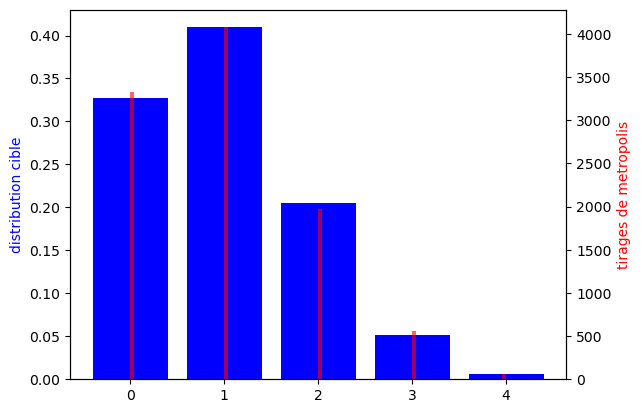
\includegraphics[scale=0.25]{loi bin.png}
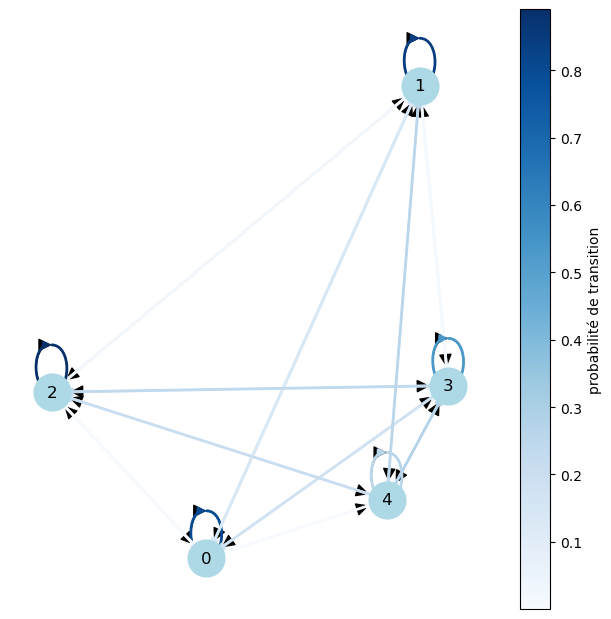
\includegraphics[scale=0.25]{loi bin graph.png}

\newpage
\paragraph{Application à une loi de Poisson :}
\begin{center}
\begin{python}
N = 15

distribution_cible = poisson(5)

# Matrice de transition uniforme de taille N*N
proposition = np.full((N,N),1/N)

tirage = hastings_metropolis_tirage(0,distribution_cible,proposition,iterations=100_000)
mk_c = markov_chain_from_tirage(tirage,N)
\end{python}
\end{center}
Résultats :

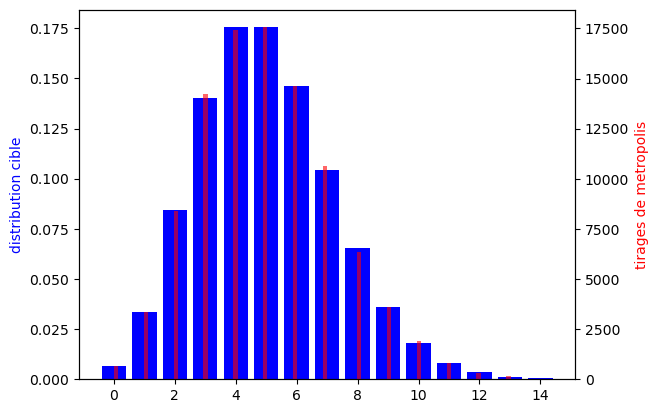
\includegraphics[scale=0.5]{poisson.png}

\newpage
\paragraph{Application à une loi uniforme :}
\begin{center}
\begin{python}
N = 15

distribution_cible = lambda k : 1/(N-2) if 0<k and k<N else 0

# Matrice de transition aleatoire
proposition = np.array([ ligne / ligne.sum()
    for ligne in [np.random.rand(N) for _ in range(N)]
])


tirage = hastings_metropolis_tirage(0,distribution_cible,proposition,iterations=100_000)
mk_c = markov_chain_from_tirage(tirage,N)
\end{python}
\end{center}
Résultats :

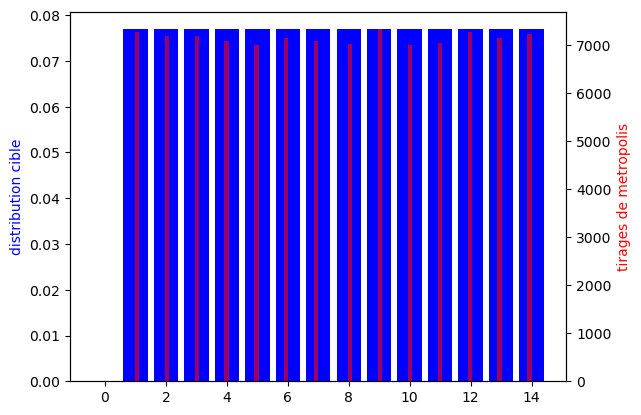
\includegraphics[scale=0.5]{uniforme.png}

\newpage
\paragraph{Application à une loi géométrique :}
\begin{center}
\begin{python}
N = 20

distribution_cible = geo(0.33)

# Matrice de transition aleatoire
proposition = np.array([ ligne / ligne.sum()
    for ligne in [np.array([abs(np.random.normal(i,1)) for _ in range(N)]) for i in range(N)]
])

tirage = hastings_metropolis_tirage(0,distribution_cible,proposition,iterations=100_000)
mk_c = markov_chain_from_tirage(tirage,N)
\end{python}
\end{center}
Résultats :

\includegraphics[scale=0.5]{géometrique.png}

\newpage
\paragraph{Application à une loi quelconque :}
\begin{center}
\begin{python}
N = 30

distribution = np.random.rand(N)
distribution = distribution / distribution.sum()

distribution_cible = lambda k : distribution[k] if k < N and 0<=k else 0

# Matrice de transition aleatoire
proposition = np.array([ ligne / ligne.sum()
    for ligne in [np.array([abs(np.random.normal(i,1)) for _ in range(N)]) for i in range(N)]
])

tirage = hastings_metropolis_tirage(0,distribution_cible,proposition,iterations=100_000)
mk_c = markov_chain_from_tirage(tirage,N)
\end{python}
\end{center}
Résultats :

\includegraphics[scale=0.5]{loi aléatoire.png}


\newpage
\subsection{Bibliographie}

\subsubsection{Documents textuels :}
\begin{itemize}
    \item Physical Based Rendering, from the theory to implementation Matt Pharr, Wenzel Jakob, Gre
    \item \url{https://fr.wikipedia.org/wiki/Chaîne_de_Markov}
    \item \url{https://dms.umontreal.ca/~bedard/BergeronL_rapport_final.pdf}
    \item \url{https://www.math.univ-paris13.fr/~tournier/fichiers/agreg/2014/cours_markov.pdf}
    \item \url{https://www.math.u-bordeaux.fr/~mchabano/Agreg/ProbaAgreg1213-COURS5-CM.pdf}
    \item \url{https://www.imo.universite-paris-saclay.fr/~pierre-loic.meliot/agreg/markov.pdf}
    \item \url{https://www.college-de-france.fr/fr/agenda/cours/apprentissage-et-generation-par-echantillonnage-aleatoire/algorithme-de-metropolis-hasting}
    \item \url{https://www.math.u-bordeaux.fr/~mibonnef/mimse-markov/recurence-transience.pdf}
    \item \url{https://perso.univ-rennes1.fr/jean-christophe.breton/agreg/AGREG/COURS/ch-mark2.pdf}
    \item \url{https://fr.wikipedia.org/wiki/Processus_stochastique}
    \item \url{https://fr.wikipedia.org/wiki/Méthode_de_Monte-Carlo_par_chaînes_de_Markov}
    \item \url{https://www.math.u-bordeaux.fr/~mchabano/Agreg/ProbaAgreg1314-COURS5-CM.pdf}
    \item \url{https://fr.wikipedia.org/wiki/Algorithme_de_Metropolis-Hastings#cite_note-2}
    \item \url{https://www.radcliffe.harvard.edu/news-and-ideas/flash-of-genius}
    \item \url{https://fr.wikipedia.org/wiki/Probl\%C3\%A8me_du_voyageur_de_commerce}
    \item \url{https://www.cambridge.org/core/journals/mathematical-proceedings-of} \url{-the-cambridge-philosophical-society/article/abs/shortest-path-through-many-points/F1C28B5730B94887F4659FCBF8A1F2BB} \\ % Document de Thomas Kirkman, Jillian Beardwood, J.H. Halton ou John Hammersley.
\end{itemize}

\subsubsection{Documents vidéos :}
\begin{itemize}
    \item \url{https://www.youtube.com/watch?v=yCv2N7wGDCw}
    \item \url{https://www.youtube.com/watch?v=MxI78mpq_44}
    \item \url{https://www.youtube.com/watch?v=e0ZHDK4DSEI&list=PLWoShwK0FEjovcc32x9LbpDTf8pquPimV}
    \item \url{https://www.youtube.com/playlist?list=PLWoShwK0FEjovcc32x9LbpDTf8pquPimV} \\
\end{itemize}

\end{document}
